
All measured values should be measured using the ranging technique discussed in this chapter.

\begin{enumerate}
\item 
\question{Start with the circuit you built in Figure~\ref{figBreadboardBeginFour}.  Measure the voltage drop across the resistor, then measure the voltage drop across the LED.  Now, measure the voltage drop across both of them (put the red multimeter lead on the left side of the resistor and the black multimeter lead on the right side of the LED).  Write down your values.}
\solution{The voltage drop across the LED should be around $1.8\myvolt$.  The voltage drop across the resistor should be around $7.2\myvolt$, but will vary with the battery's current voltage (i.e., how new or old it is).  However, the voltage drop across both of them should be exactly the two of them added together (around $9\myvolt$).}
\item 
\question{Using the same circuit, change the LED from red to blue.   Measure the values again and write them down.  Measure the current going through the circuit using any wire.  Is it the same or different than before?}
\solution{With a blue LED, the voltage drop across the LED should be around $3.3\myvolt$.  The voltage drop across the resistor should be around $5.7\myvolt$, and the voltage drop across both of them should be your two results added together.  The current should be at $5.7\mymamp$.  This should be the case no matter where you test the current.}
\item 
\question{Add another LED in series with the one you have already.  Measure the voltage drops between each side of each component in the circuit.  Measure the current going through any given wire.  Write down each value.}
\solution{This will vary with the color of the LED.  However, in general, it should drop the voltage another $1.8--3.3$ volts.  It will also reduce the current flowing through the circuit.  However, all wires should have the same current going through them.}
\item 
\question{Take the new circuit you built in the previous problem and draw the schematic for the circuit.}
\solution{This may vary a little, but should look something like this:
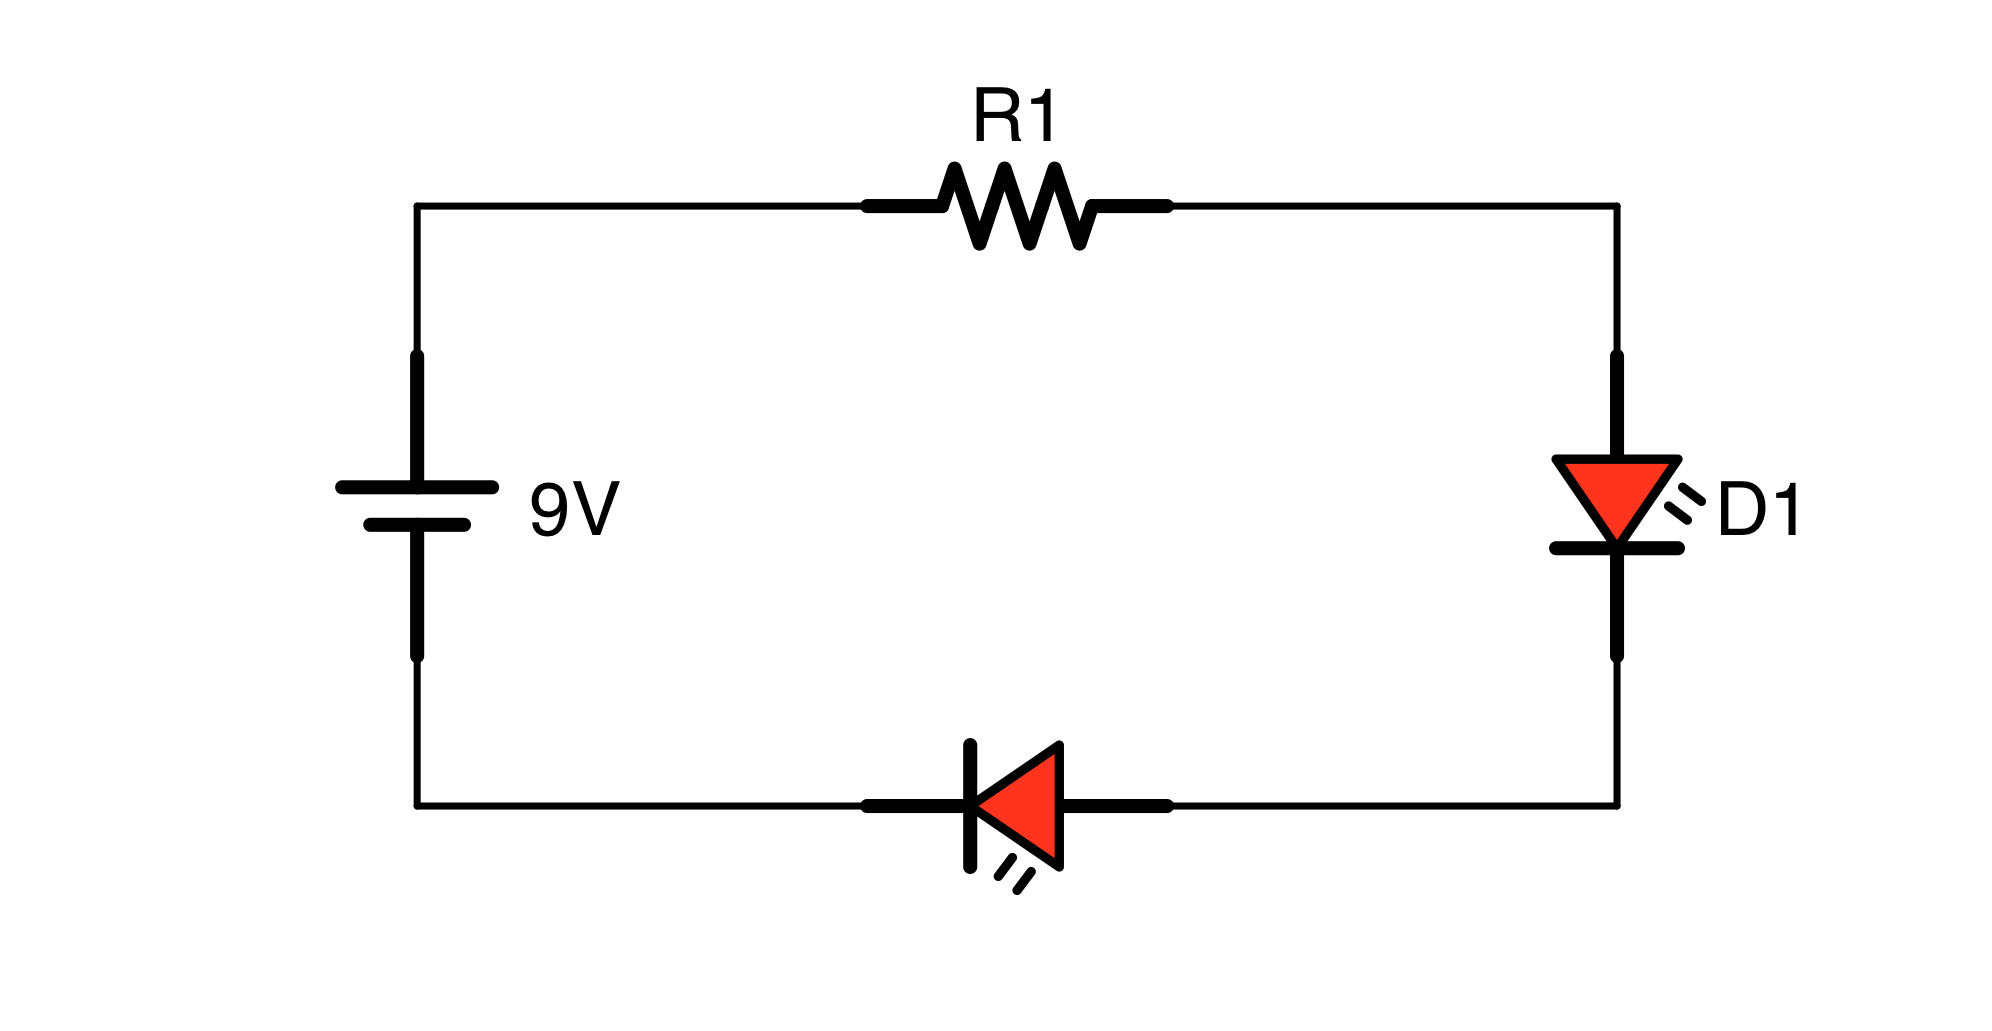
\includegraphics[width=\columnwidth]{SolutionTwoLED.png}
}
\end{enumerate}
